% Version 2020-01-06
% update – 161114 by Ken Arroyo Ohori: made spacing closer to Word template throughout, put proper quotes everywhere, removed spacing that could cause labels to be wrong, added non-breaking and inter-sentence spacing where applicable, removed explicit newlines
% update – 010819 by Dennis Wittich: made spacing and font size closer to Word template, updated references and refernces style
% update – 042319 by Dennis Wittich: font size of captions set to 'small', first author names are shortened, hyphenation fixed
% update – 010620 by Dennis Wittich: Footnotes alignment set to left

\documentclass{isprs} % isprs class modified 23-04-2019 (Dennis Wittich)
\usepackage{subfigure}
\usepackage{setspace}
\usepackage{geometry} % added 27-02-2014 Markus Englich
\usepackage{epstopdf}
\usepackage{natbib}
\usepackage{tabularx}
\usepackage{booktabs}
\usepackage[colorlinks, allcolors=blue]{hyperref}
%\bibliographystyle{apalike}
\usepackage[labelsep=period]{caption}  % added 14-04-2016 Markus Englich - Recommendation by Sebastian Brocks
\usepackage[british]{babel} 
\usepackage[hang]{footmisc}
\def\footnotemargin{1em} % added 08-01-2020 Dennis Wittich
\usepackage{fancyref}

%\usepackage[authoryear]{natbib}
%\def\bibhang{0pt}

\geometry{a4paper, top=25mm, left=20mm, right=20mm, bottom=25mm, headsep=10mm, footskip=12mm} % added 27-02-2014 Markus Englich
%\usepackage{enumitem}

%\usepackage{isprs}
%\usepackage[perpage,para,symbol*]{footmisc}

%\renewcommand*{\thefootnote}{\fnsymbol{footnote}}
\captionsetup{justification=centering,font=normal} % thanks to Niclas Borlin 05-05-2016
\captionsetup[figure]{font=small} % added 23-04-2019 Dennis Wittich
\captionsetup[table]{font=small} % added 23-04-2019 Dennis Wittich

% Location of the images
\graphicspath{{figures/}}

\begin{document}

\title{Assessing Digital Elevation Models with different image overlap using photogrammetry}

% KAO: Remove extra spacing
\author{Robert van de Vlasakker}

% KAO: Remove extra newline
\address{} % Not needed

% If the corresponding author is NOT the final author, always add a % space before the subsequent comma, i.e.
% first author name\textsuperscript{a,}\thanks{Corresponding author} , % second author name \textsuperscript{b}, etc.
% thanks to Niclas Borlin 05-05-2016

% BB: leave these empty, but do not delete
\commission{}{} %This field is optional.
\workinggroup{} %This field is optional.
\icwg{}   %This field is optional.

% KAO: Use times symbol
\abstract{
Photogrammetry is easy to use these days and can be used to create a digital elevation models (DEM) of an area. 
Image overlap plays an important role in the process of photogrammetry.
A high overlap takes more time to gather in the field and takes longer to process.
Less overlap usually results in a less accurate calculations. 
In this paper the overlap of an area is artificially reduced and digital elevation models have been created with different image overlaps.
The digital elevation models are compared to see how reducing the image overlap influences the result. 
When the absolute values of the DEM in compared large differences are visible.
However, when the scaled DEM's are compared in a boxplot the differences appear to be minimal.
Finally a violin plot has been made of the complete image set DEM minus the reduces image set DEM's.
The more images are used, the more the difference of the DEM's is centered around 0.
The DEM of the dataset with the highest images count seems to be the most similar to the DEM of the full dataset.
}

\keywords{Photogrammetry, Digital Elevation Model, Image Overlap, Agisoft Metashape}

\maketitle

%\saythanks % added 28-02-2014 Markus Englich

\section{Introduction}\label{Introduction}

Photogrammetry is the process of reconstructing spatial information with images through computer vision. 
These days most photogrammetry data is acquired with unmanned aerial vehicles (UAV) \citet{UAVAreMoreUsed}. 
UAV's come with GNSS and provide high resolution images needed for photogrammetry.
The process uses similar points visible on multiple images to determine the points in 3D space.
The reconstruction certainty of these points is strongly dependent on the overlap between different images. 
Because most programs handle 2D data better than 3D data, the point cloud is usually used to build a digital elevation model (DEM) \citet{DemIncrease1}.

A higher image overlap results in more similar image points which will increase the reconstruction certainty of the points \citep{MoreOverMoreAcc}.
A higher image overlap, does not automatically results in a denser point cloud. \citep{EffectofUABimgcamover}. 
A high overlap is needed in complex structures like vegatetion; if parts of the object are not visible on the image, they will not be reconstructed in the point cloud \citep{AccessingImageOverlap}.
However, an image dataset with a high overlap takes longer to gather, and may results in multiple drone flights for a single dataset \citep{UAVpopularity}.
In the reconstruction process, a high overlap will also result in longer computation time \citep{AccessingImageOverlap}
By reducing the image overlap, time and computing power may be saved without loosing too much spatial information.
This main goal of this study is to investigate how different image overlap influence the DEM result that is created with photogrammetry. 





\section{Materials and Methods}

\subsection{Study Area}\label{sec:Study Area}
The data covers an area in Ghana, about 20km south east of Ejura (lat. 7.3064212, lon. -1.164493). 
The area of interest is about 25000 m\textsuperscript{2}. 
The area consists mostly of savanna area.
There are a few trees present on the observed location.
\begin{figure}[h]
    \centering
    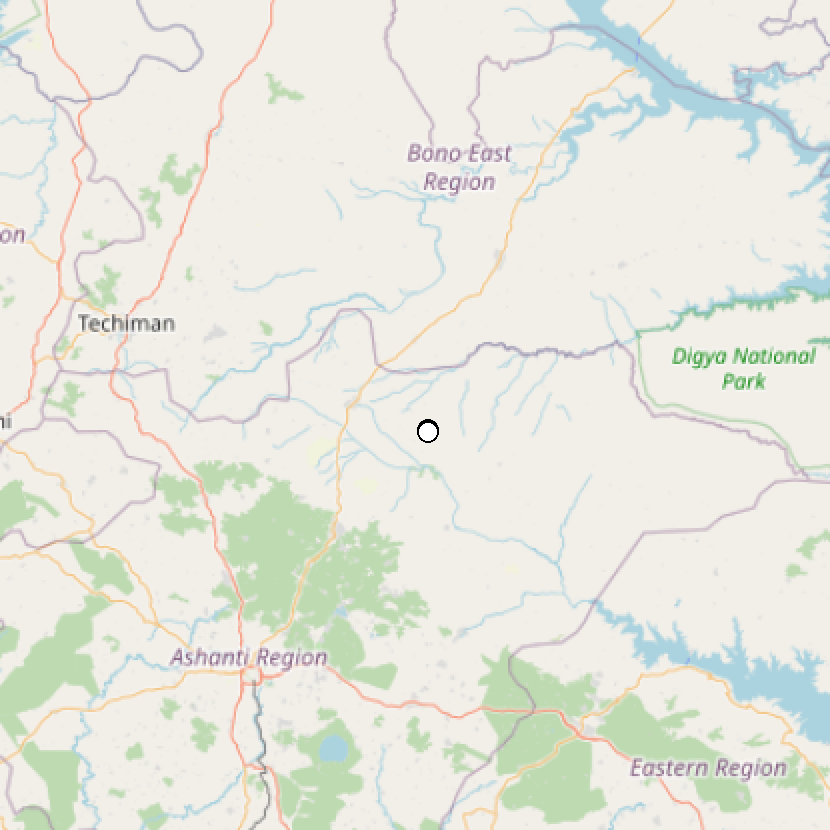
\includegraphics[width=4cm]{locationwide.png}
    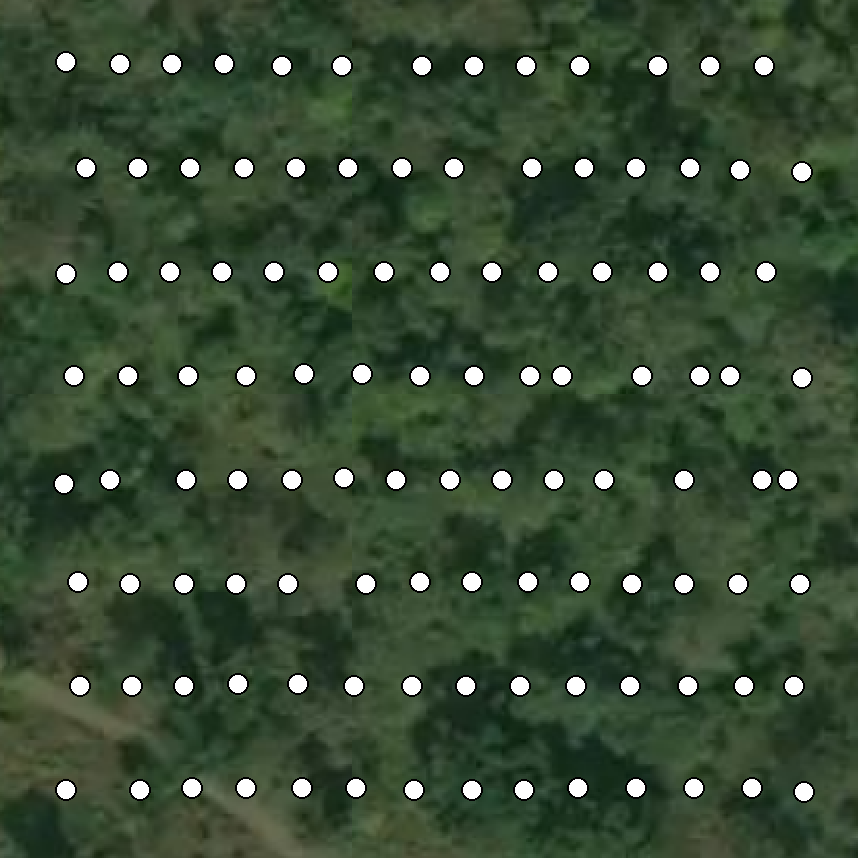
\includegraphics[width=4cm]{imgloc.png}
    \caption{Area of Interest and Unprocessed Image GPS Locations}
    \label{fig:areaofinterest}
\end{figure}
Each image has a resolution of 4000 times 3000 and was taken by a DJI Phantom 3.
The images all contain GNNS location (WGS84). 
The complete data set consists of 111 images.
Their exact location can be found in figure \ref{fig:areaofinterest}.


\subsection{Image Processing}
For image processing and DEM generation Agisoft Professional edition 1.6.5 (Agisoft LLC., St. Peterburg, Russia) was used \citep{AgisoftMetashape}.
All data have been processed on the cloud service provided by Agisoft (\url{https://cloud.agisoft.com}).
The cloud processing is done on 32 vCPU's (Intel Xeon E5 2686 v4) with two NVIDIA Tesla M60 GPU's and 240 GB of RAM.

First, the complete data set has been aligned on medium quality.
Next, the dense cloud was built on medium quality (no depth filtering), resulting in a dense cloud of 3,268,264 points.
A mesh was built using the the triangulated irregular network (TIN) algorithm by \citet{axelsson1999processing}. 
finally after the mesh the Reduce Overlap function was used to reduce the amount images used in the process of photogrammetry. 
The mesh was set to create a 2.5D height field.

\textbf{Reduce Overlap.} 
The algorithm of the Reduce Overlap function tries to select a minimal amount of images such that each point of the model is observed from N locations/angles.
If a point is observed multiple times from the same location/angle, than this still counts as one. 
The exact algorithm and parameters behind the Agisoft Reduce Overlap function are unknown.
The input dataset was a 2.D height field mesh. 
Because in this paper the comparison will be made with a DEM, a height field was computed.
In Agisoft Metashape the 'Reduce Overlap' had three different settings, low, medium and high. 
All of the settings are used and the remaining images are used for further processing.
In \ref{tab:ImageProcessing} the amount of images for each Reduce Overlap setting can be found.

\textbf{Camera Locations.}
In figure \ref{fig:cameralocation} the estimated camera locations can be found. The estimated camera location is estimated by the image processing alogrithm of Metashape.
The images are matched based on an adapted version of the SIFT algorithm \citep{lowe1999object, AgisoftMetashape}. 

\begin{figure}[h]
    \centering
    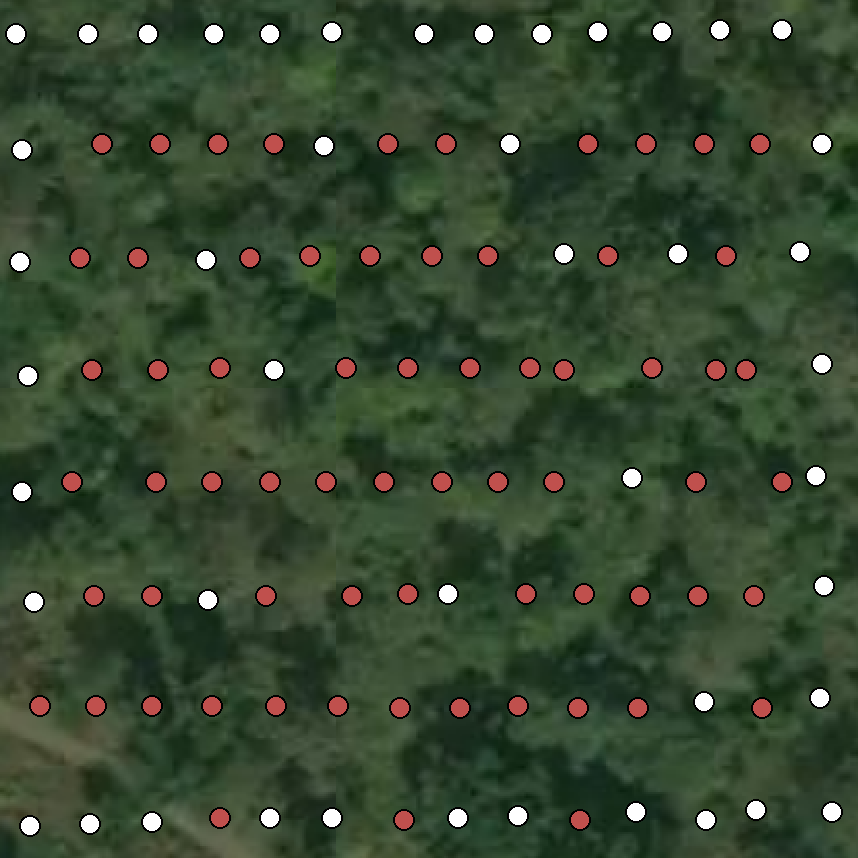
\includegraphics[width=1.9cm]{loc_low.png}
    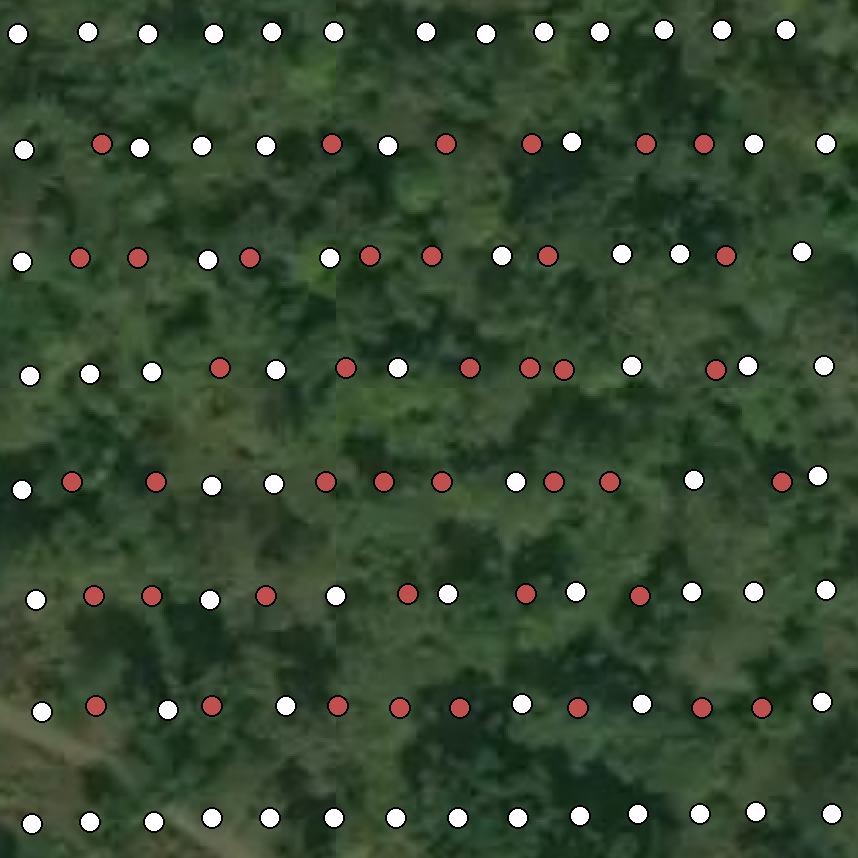
\includegraphics[width=1.9cm]{loc_med.png}
    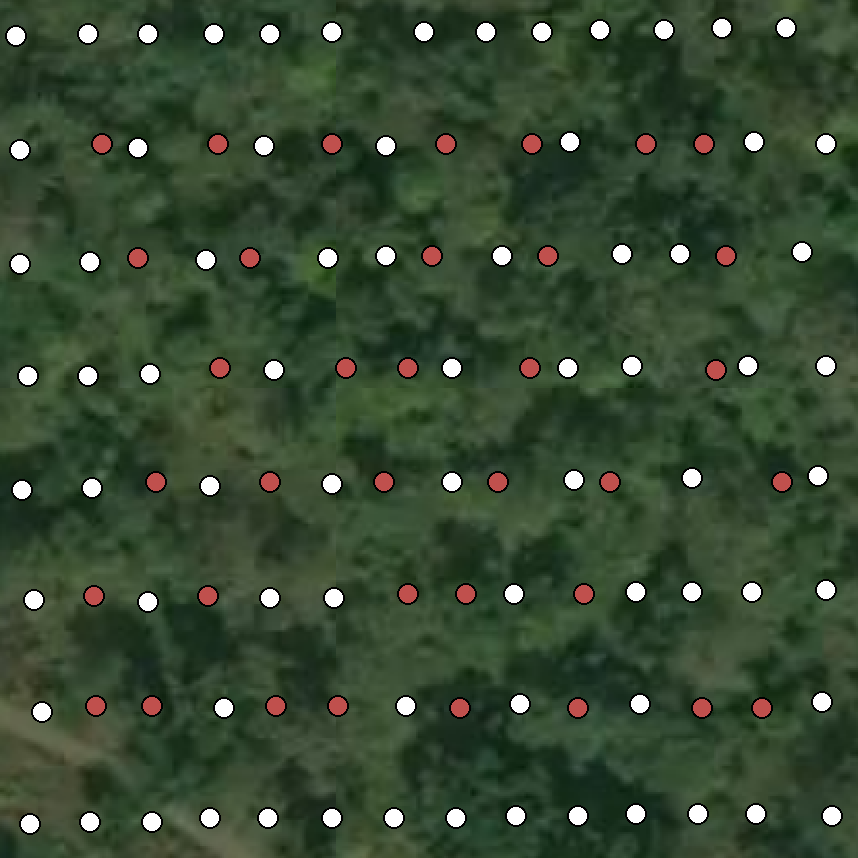
\includegraphics[width=1.9cm]{loc_high.png}
    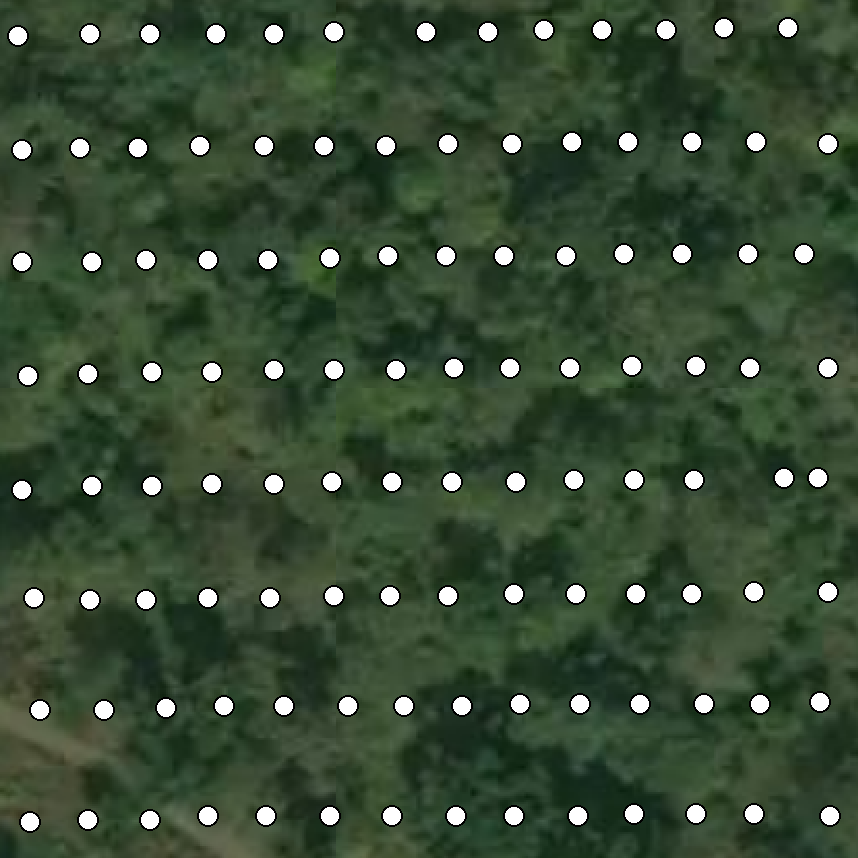
\includegraphics[width=1.9cm]{loc_full.png}
    \caption{Estimated camera location. 
    White: used in the image processing, red: disabled in the image processing.\\
    Clockwise (starting left top): low, medium, high and full settings}
    \label{fig:cameralocation}
\end{figure}

After the amount of images have been reduced, the data have been processed on medium for the image alignment and on medium without depth filtering for the dense cloud creation.
In table \ref{tab:ImageProcessing} an overview of the image processing results can be found.

\begin{table}[h]
    \centering
    \caption{Image Processing Results}
    \begin{tabular}{@{}cccc@{}}
    \toprule
    \textbf{Setting} & \textbf{Images} & \multicolumn{1}{l}{\textbf{Sparse Cloud}} & \multicolumn{1}{l}{\textbf{Dense Cloud}} \\ \midrule
    -      & 111 & 80,901 & 3,269,264 \\
    Low    & 44  & 37,886 & 4,172,783 \\
    Medium & 70  & 54,556 & 3,313,399 \\
    High   & 75  & 49,692 & 3,276,832 \\ \bottomrule
    % Add processing time!
    \label{tab:ImageProcessing}
\end{tabular}
\end{table}

For all the different settings the processing time can be found in table \ref{tab:processingTime}

\begin{table}[h]
    \centering
    \caption{Processing time in seconds for the difference steps in the process.}
    \label{tab:processingTime}
    \begin{tabular}{@{}cccc@{}}
    \toprule
    \textbf{Setting} & \textbf{Sparse Cloud} & \multicolumn{1}{l}{\textbf{Dense Cloud}} & \multicolumn{1}{l}{\textbf{DEM}} \\ 
    \midrule
    -      & 150 & 292 & 17 \\
    Low    & 59  & 443 & 16 \\
    Medium & 83  & 147 & 17 \\
    High   & 129 & 159 & 17 \\ \bottomrule
\end{tabular}
\end{table}

\textbf{DEM.}
The source data for the DEM's are the dense cloud results. 
The Dense Cloud contains about the same amount of points with the exception for the lowest Reduce Overlap setting.
This setting has resulted in the dense cloud with the most points.
The TIN algorithm is used to built the DEM's \citep{axelsson1999processing}.
The image overlap is now changed, therefore the DEM's have a slightly different extent.
Because of this the largest common extent of the DEM's will be used to crop the DEM's resulting in four DEM's with an equal extent.
The DEM's will be exported from Agisoft Metashape with the same pixel resolution of 17.5 cm per pixel (1670 x 1290 pixels). 
The DEM's will also be scaled to check the differences between the DEM's without looking at the absolute values.
The scaling will be done by subtracting the mean and dividing by the standard deviation.
For further comparison all of the DEM's will be subtracted from the full model DEM.
This will result in three new DEM's that contain differences instead of height values.


\section{Results}
In figure \ref{fig:DemPlot_unscaled} are visualized using the same color range. 
In this figure the DEM's do no look similar at all.


\begin{figure}[h]
    \centering
    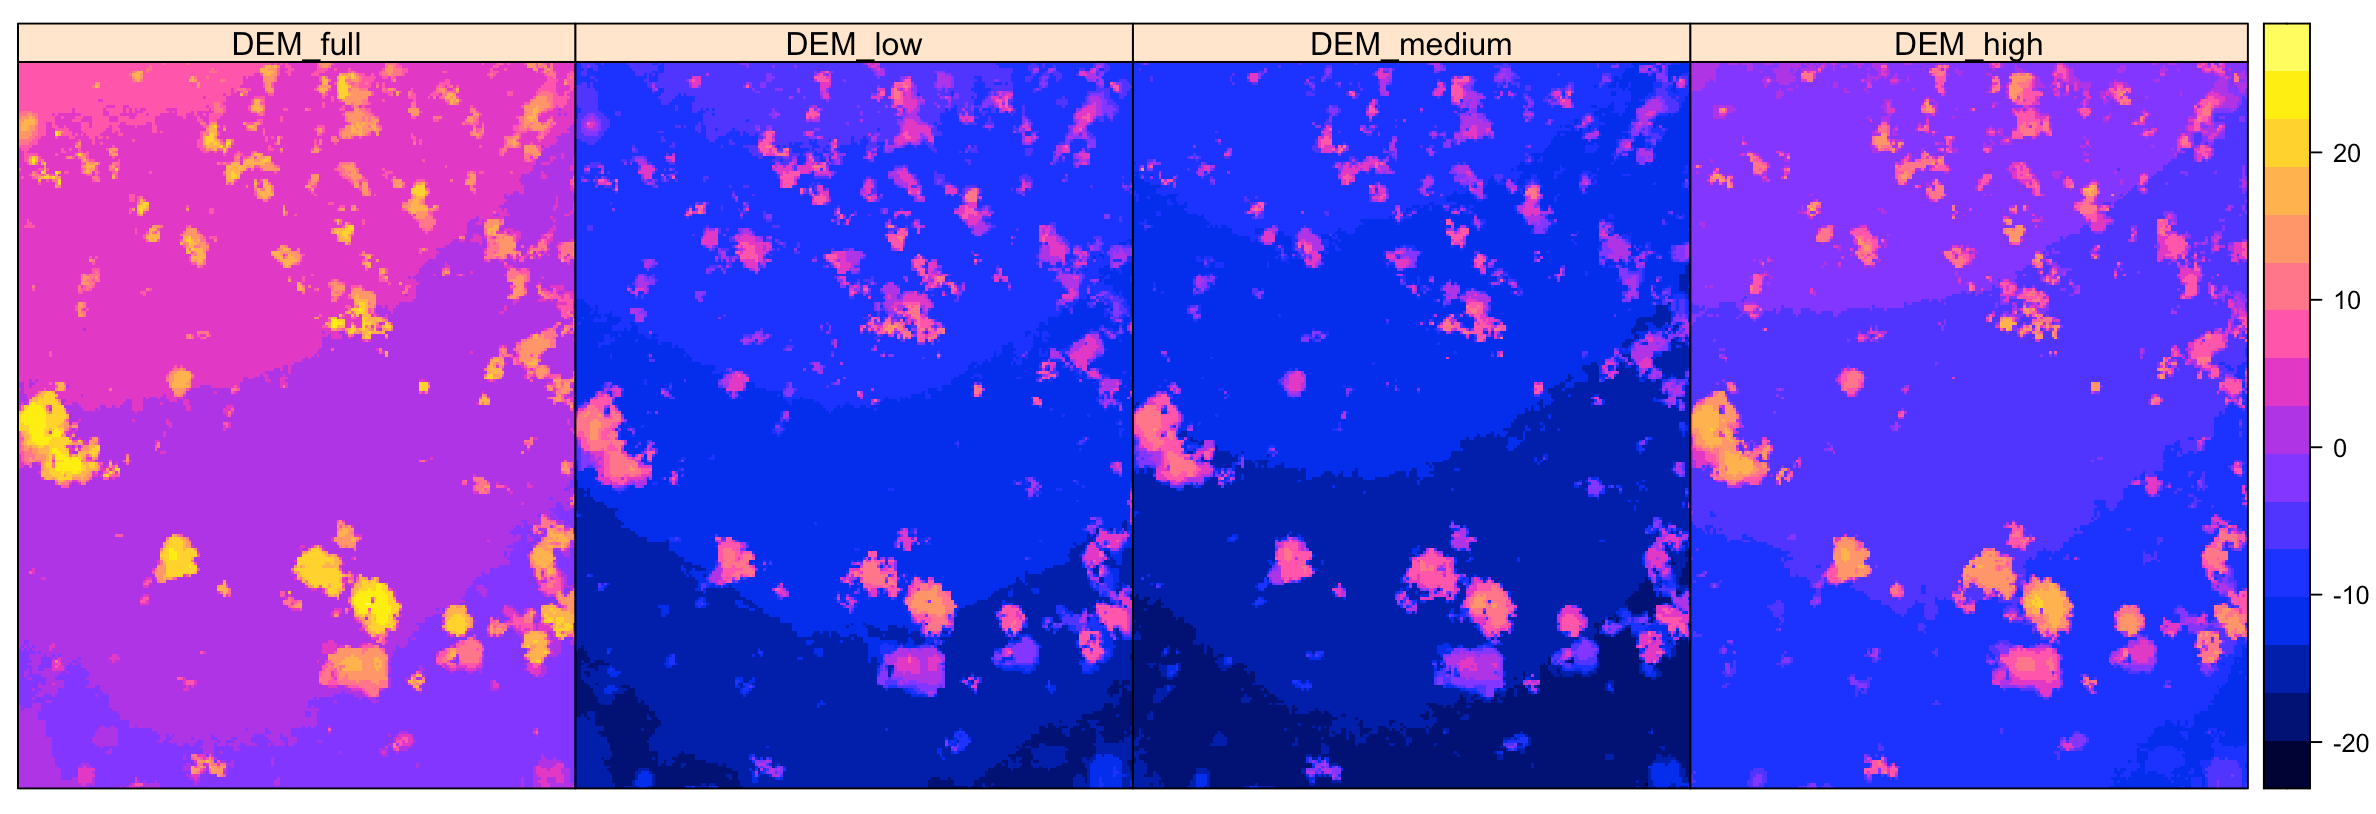
\includegraphics[width=8cm]{DemPlots.png}
    \caption{DEM Results of the Reduce Overlap}
    \label{fig:DemPlot_unscaled}
\end{figure}

As can be seen from figure \ref{fig:BoxPlot_unscaled} the DEM's are indeed different from each other. 
The outliers in the boxplot figure are probably the vegetation that is present in the area.
%For the low setting the DEM values range from -19.4 to 19.0, for the medium setting the values range from -22.7 to 16.2, for the high setting the values range from 13.1 to 20.0 and for the full model from -4.8 to 28.9.

\begin{figure}[h]
    \centering
    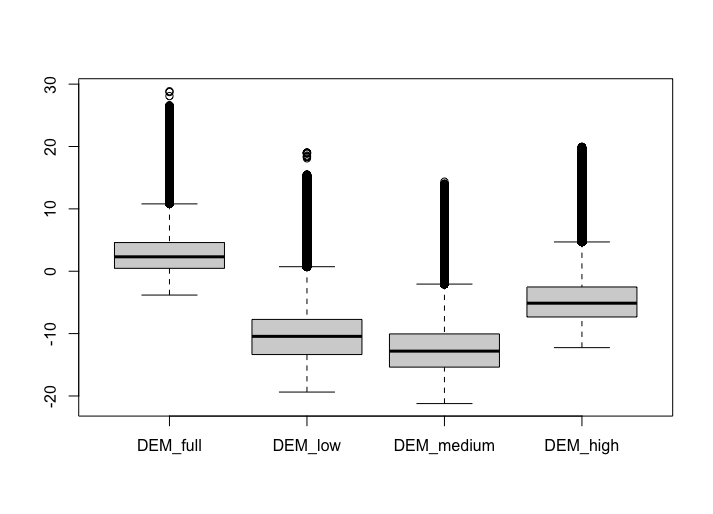
\includegraphics[width=8cm]{DemBoxplot.png}
    \caption{Box plots of the DEM Results of the Reduce Overlap}
    \label{fig:BoxPlot_unscaled}
\end{figure}

Figure \ref{fig:DemPlot_scaled} contains the same visualization of DEM plots, only for all the DEM's the data has been scaled.

\begin{figure}[h]
    \centering
    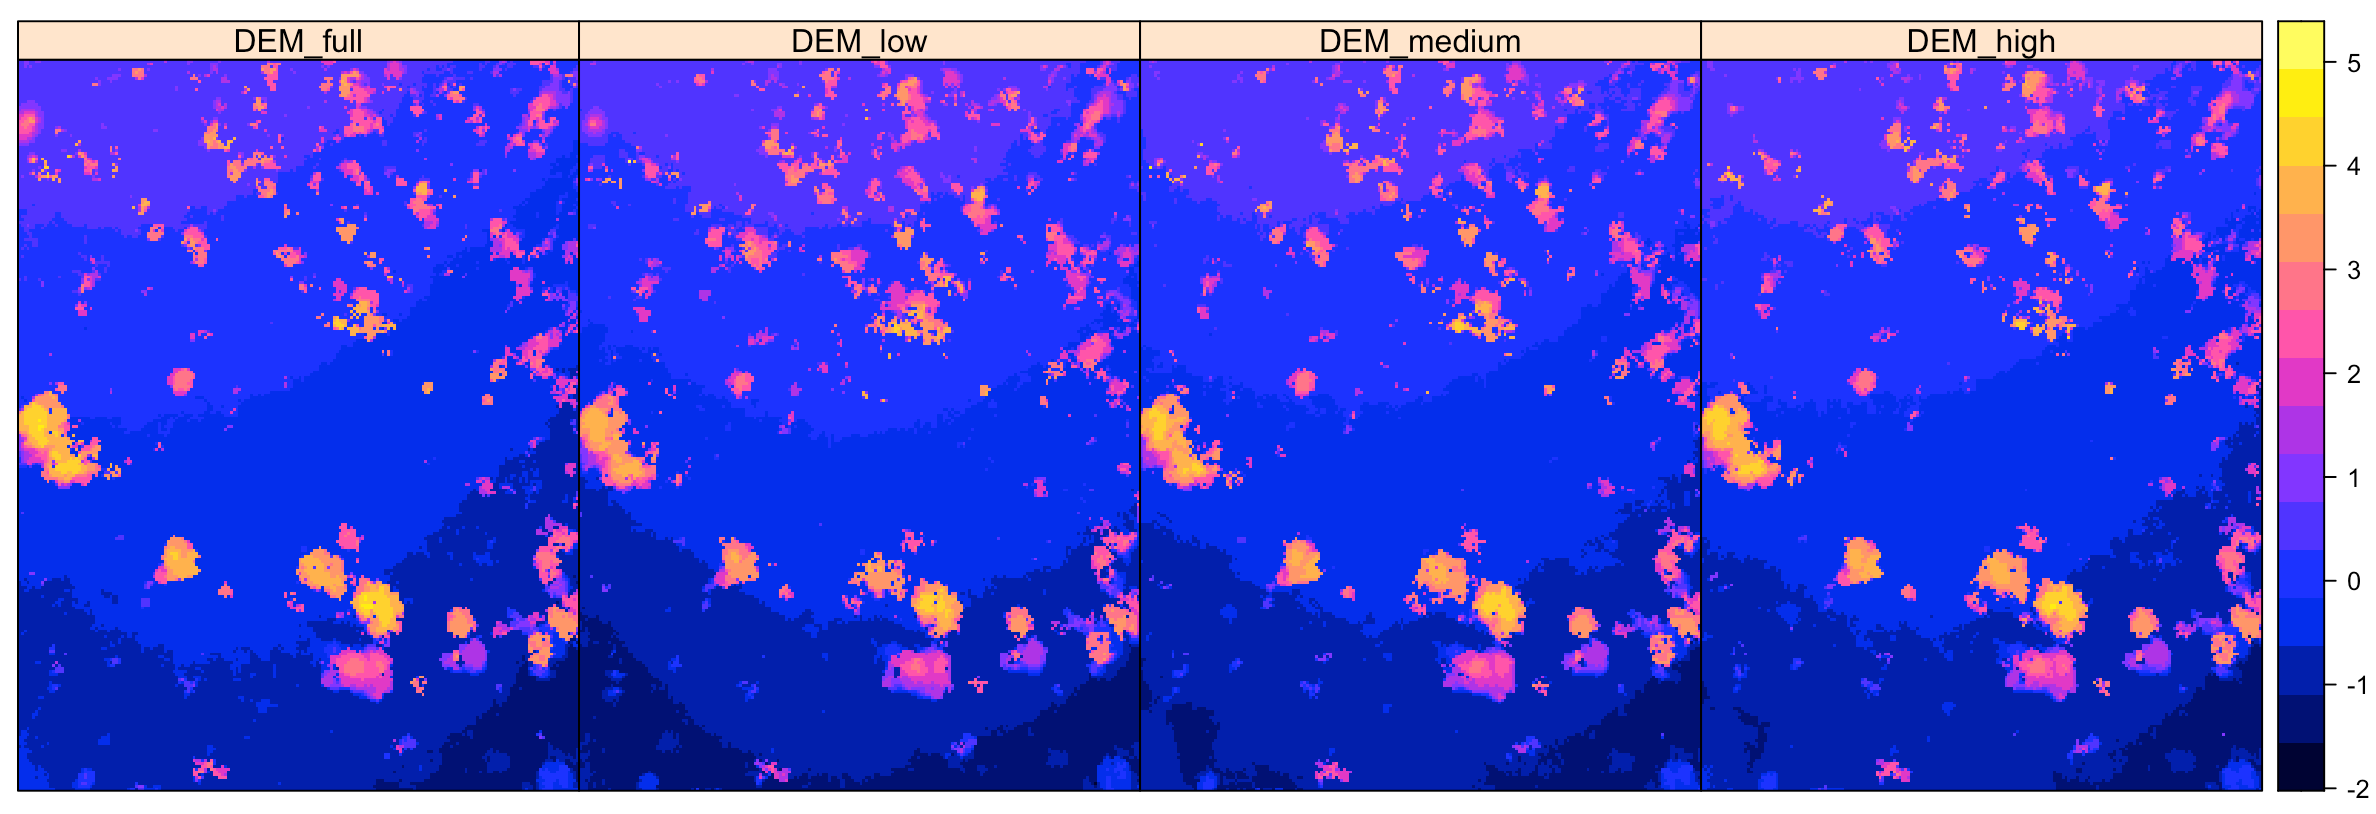
\includegraphics[width=8cm]{DemPlots_scaled.png}
    \caption{Scaled DEM Results of the Reduce Overlap}
    \label{fig:DemPlot_scaled}
\end{figure}

The same applies for figure \ref{fig:BoxPlot_unscaled}, only now the boxplot contain the scaled data values.

\begin{figure}[h]
    \centering
    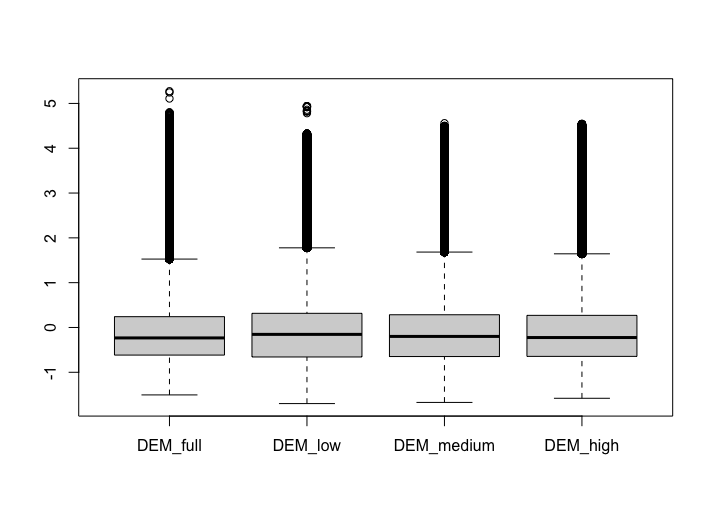
\includegraphics[width=8cm]{DemBoxPlot_Scaled.png}
    \caption{Scaled DEM Results of the Reduce Overlap}
    \label{fig:BoxPlot_scaled}
\end{figure}

In figure \ref{fig:ViolinPlot} a violin plot containing the difference of the DEM between the different Reduce Overlap settings can be found. 
It is visible that the overall error of the scaled DEM's varies from around -5.0 to 5.0.
For the high settings, the differences are more centered around zero, while this is not the case for low and medium settings.
For medium setting the difference is slightly more centered around 0.0 than low settings.

\begin{figure}[h]
    \centering
    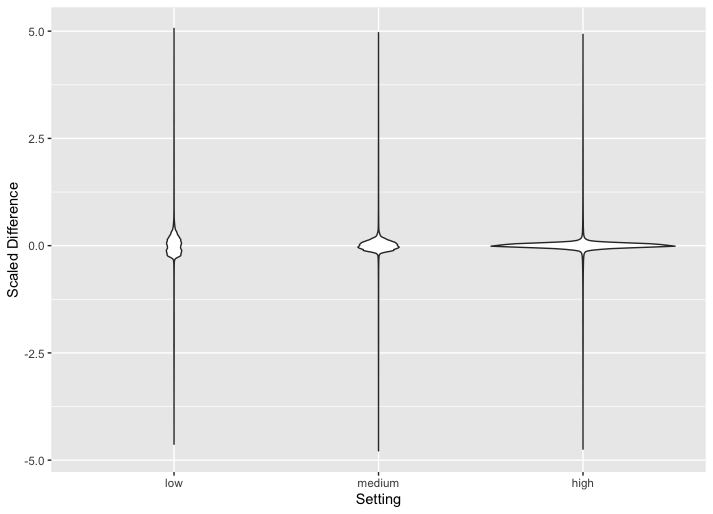
\includegraphics[width=8cm]{ViolinPlotOrdered.png}
    \caption{Violin plot of the difference between the full DEM and the reduced DEM's. All violin plots contain 2.154.300 measurements (DEM rows x DEM columns}
    \label{fig:ViolinPlot}
\end{figure}

% Substract the DEM from each other

\section{Discussion}
The goal of this research was to assess the difference between DEM's of the same area with different image overlap. 
The image reduction in the paper was calculated in Agisoft Metashape with the Reduce Overlap function.
The amount of images used in the processing does not seem to influence the density of the dense cloud, which was also concluded by \citet{EffectofUABimgcamover}.
In this research the point confidence was not measured, the dense cloud were directly used to construct a DEM. 

The input mesh for the Reduce Overlap was a 2.5D height field. 
With more complex objects that need to processed as a real 3D object the amount of dense cloud may decrease if the amount of images is reduces significantly.
Because the mesh was structured as a 2.5D surface, difficult points were removed from the model, e.g. in this case the tree structures were lost in the process.
An other option is that the Reduce Overlap function will not have much influence on the image count.

There is a large different between the absolute values between the different DEM's, this can be seen visually in figure \ref{fig:DemPlot_unscaled} and also when comparing the boxplot values in figure \ref{fig:BoxPlot_unscaled}.
With the use of at least three ground control points the error in the absolute values of the can be reduced \citep{AssessingUAVGCPS, GCPbetterAccuracy, GeoreferencedPointClouds}.
Using GCP's in the different image dataset will reduce the absolute error.

The violin plots indicate that the dataset with the highest image count is most similar to the full dataset; the difference of is more centered around zero, while the two lower image count datasets are more widespread (higher SD).
The largest errors difference (around -5/5) between the scaled DEM seem to be the same for all the image datasets.
The modelling software probably has difficulties in modelling the complex structures of the vegetation, resulting in a larger difference when the image count is lower.
This could result in more error around vegetation canopies where the algorithm has difficulties in accurately measuring the height.
An other option may changing the filtering setting provided by the Metashape dense cloud generation.
In this research no depth filtering was used, by applying a more aggressive filtering technique the complex structures of the vegetation will be lost in the DEM generation \citep{AgisoftMetashape}.
Further research is needed to see where this differences exactly occur and if a different depth filtering may result in different results.

\section{Conclusion}
Using different image overlap in the same area results in DEM's with different absolute values.
The two image dataset with the least images show the largest difference in absolute value range compared to the original dataset with all images. 
The image dataset with the highest image count, has a DEM that is most similar compared to the original dataset.
When the scaled values are compared there seems to be a minimal difference between the DEM's.
If more images are used in the dataset, the difference between the scaled DEM's compared to the full images set becomes smaller; the DEM differences are more centered around 0.


% KAO: Sloppy spacing ensures non-overfull lines. Can be removed if this is not an issue.
\sloppy




{
	\begin{spacing}{1.17}
		\normalsize
		\bibliography{bibliography} % Include your own bibliography (*.bib), style is given in isprs.cls
	\end{spacing}
}



\vspace{1cm}
\end{document}





Photogrammetry is the process of reconstructing spatial information with images through computer vision. 
The process uses similar points visible on multiple images to determine the points in 3D space.
The reconstruction certainty of these points is strongly dependent on the overlap between different images. 
When a point is visible on more images, the reconstruction certainty will be higher \citep{MoreOverMoreAcc}.
This is especially the case with the reconstruction of irregular formed object like vegetation \citep{AccessingImageOverlap}.
With irregular objects, a higher overlap is preferred to capture each side of the object.
If parts of the object are not visible on the image, they will not be reconstructed in the point cloud.
In the reconstruction process, a high overlap will also result in longer computation time \citep{AccessingImageOverlap}
However, a higher image overlap, does not automatically results in a denser point cloud. \citep{EffectofUABimgcamover}. 
These days most photogrammetry data is acquired with Unmanned Aerial Vehicles (UAV) \citet{UAVAreMoreUsed}. 
UAV's come with high resolution cameras, GNSS and are available almost anywhere these days.
While UAV's do come with high resolution sensors and are relatively cheap, small, high capacity batteries are not available \citep{UAVpopularity}.
A high image overlap takes longer to gather than a low image overlap. 
A drone can use a higher altitude so the sensor captures a larger area.
however, with a higher flight altitude the detail of the image will be less than that of a drone with a lower flight altitude.
This way the gathering process takes longer, and the UAV might even need to switch batteries instead of taking the images in a single flight.
By reducing the image overlap, time and computing power may be saved without loosing too much spatial information.
This main goal of this study is to investigate how different image overlap influence the DEM result that is created with photogrammetry. 